% Intended LaTeX compiler: pdflatex
\documentclass[10pt,a4paper,UTF8]{article}
\usepackage{zclorg}
\usepackage{tikztheorem}
\author{zcl.space}
\date{}
\title{中心极限定理}
\hypersetup{
 pdfauthor={zcl.space},
 pdftitle={中心极限定理},
 pdfkeywords={probability},
 pdfsubject={},
 pdfcreator={Emacs 25.0.50.1 (Org mode 9.0.6)},
 pdflang={English}}
\begin{document}

\maketitle
\tableofcontents
\titlepic{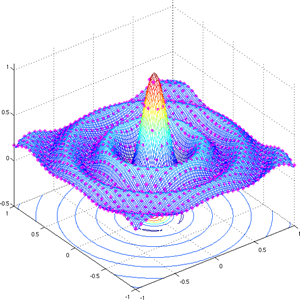
\includegraphics[scale=0.25]{../../img/sinc.PNG}}

\section{引言}
\label{sec:org5e1ec81}


中心极限定理是概率论中最著名的定理之一。不太严格的说,中心极限定理认为大量独立随机变量的和近似服从高斯分布。因此中心极限定理不仅提供了计算独立随机变量和的有关概率的近似值的简便方法,同时也帮助解释了现实世界中许多实际的总体分布的频率曲线呈现钟形曲线的原因。
\section{证明}
\label{sec:orge7a0ec9}


\begin{tikztheorem}
设\(X_{1},\ldots ,X_{n},\ldots\)为独立同分布的随机变量序列,其公共分布的均值为\(\mu\),方差为\(\sigma^{2}\),则随机变量:
\begin{equation}
\label{eq:1}
\frac{X_{1} + \ldots + X_{n} - n\mu}{\sigma \sqrt{n}}
\end{equation}
的分布当\(n\to \infty\)时趋向于标准正态分布。即对任何\(-\infty < a < \infty\)
\begin{equation}
\label{eq:2}
P\bigg\{ \frac{X_{1} + \ldots + X_{n} - n\mu}{\sigma\sqrt{n}} \leq a \bigg\} \to \frac{1}{\sqrt{2\pi}}\int_{-\infty}^{a}e^{-x^{2}/2}dx \quad n\to \infty
\end{equation}
\end{tikztheorem}

我还没有完全看懂。留待以后证明
\end{document}
